\section{密教}
所謂密教(Esoteric Buddhism),世界學者一般通稱為怛特羅(Tantra)佛教,也有稱為真言乘(Mantra-yāna)、持明乘(Vidyā-dhara-yāna)、密乘(Esoteric-yāna)、果乘(Phāla-yāna)、金剛乘(Vajra-yāna)等。
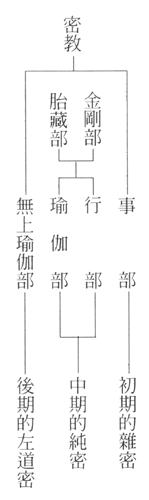
\includegraphics[scale=0.3]{释家/images/密教.png}
\paragraph{根據西藏所傳的密教} 分為四部:1.事部,2.行部,3.瑜伽部,4.無上瑜伽部。
\paragraph{中國舊傳的密乘傳入日本的} 分為兩部:1.金剛部,2.胎藏部。
\paragraph{近代學者將歷史上的密教分為三期} 1.初期的雜密,2.中期的純密,3.後期的左道密。
密教與顯教相對,是大乘佛教的判別。顯教是如來應化身(釋迦)的逗機方便說法,密教是如來報身(大日)的祕奧真實說法;顯教說歷三大阿僧祇劫修菩薩行而後成佛;密教則依於大日如來自受用報身所說內證自覺聖智之法,及大普賢金剛薩埵他受用報身之智,現生遇到曼荼羅阿闍梨,乃至灌頂受金剛之名號,由此而得甚深不可思議法,超越二乘聖者及十地菩薩,即身成佛。

\subsubsection{密教四部}
\begin{itemize}
  \item 事部:即是雜密,亦稱作密,其修無相瑜伽,即妄以明空性之理,常我的色彩尚不濃。
  \item 行部:亦稱修密,此部以《大毘盧遮那成佛神變加持經》(即《大日經》)(《大正藏》一八‧一頁中)為主,以《大日經‧住心品》中的:「菩提心為因,悲為根本,方便為究竟」三句為根本。又講十緣生,頗類於《般若經》的性空之說;但在「菩提心」的心中,已帶有常我的色彩。以大悲為本,以隨機的方便而度眾生,實在是表現了大乘佛教的偉大特色。
  \item 瑜伽部:瑜伽部配合行部的方便為究竟而融攝世俗,故以如來做在家相(天人相)的大日為其中心,以金剛手等為其護翼,出家相的釋迦及二乘聖者,被置於外圍,此由胎藏界及金剛界的曼陀羅(Mandala 密壇,修密法的道場),即可以明白。這在理論上,是因大日如來為報身佛,是化身釋迦佛的本尊,本尊應居中心;在實際上,是圓融了外教的群神,且以外教的群神,均為本尊方便攝化的顯現,所以,印度一切的善神惡神,都為密教所攝。由降伏的意念轉為崇拜的意念,乃係出自事事無礙的即事而真,所以本尊應該是在家菩薩相。
  \item 無上瑜伽部:這是最高的密法,此法修成,便是即身成就的佛,故在今日的西藏黃教,視無上瑜伽為最難修持的密法。
\end{itemize}

\subsection{灭亡}
佛教之在印度滅亡,有兩大因素:一是佛教自身為了迎合印度的外道,結果也變成了與外道合流而使自己融入於印度教中。二是回教軍隊的屢次入侵與徹底摧毀,而使佛教沒有了容身之地。
